%!TEX root = ../Master.tex
\section{Introduction}\label{sec:introduction}
%Why is the topic of interest?
	The popularity of drones has increased in recent years due to their applicability in a broad spectrum of scenarios in different fields. Particularly, live video streaming has shown to be of interest in search and rescue, law enforcement, military operations, industrial usage and entertainment\cite{lockheed}, as shown in Figure \ref{fig:drone}.
	In several of these applications, there are strict delay requirements regarding the video stream, e.g. in military operations delayed information of the enemies position can have severe consequences.
%What is the background on the previous solution?
	A reliable video stream to multiple receivers can be achieved with unicast if the group size and the amount of video data does not exceed the capacity of the wireless channel. To improve reliability during unicast the transmission rate is adapted based on feedback from the receiver gaining different properties in terms of noise sensitivity and throughput. To account for packet erasures a reliable transmission protocol can be used.

	If the capacity of the wireless channel is exceeded due to an increased amount of receivers, multicast can be used to service the group. However, multicast is not without challenges. Current standardized protocol stacks do not implement feedback mechanisms for multicast. Therefore, the MAC layer is unable to adapt to changes in channel conditions. %The common implementation is to use the lowest data rate possible, since this is the least sensitive transmission scheme. 
The lack of feedback is also problematic at the transport layer, where only connectionless protocols support multicast, which means that packet erasures are unhandled. The specific multicast technology examined in this paper is IEEE 802.11 \cite{IEEE80211g}.

%What is the background on potential solutions?
	For most video codecs, data loss is not acceptable as losses degrade quality and in the worst case, the video becomes unplayable. Therefore, plain 802.11 multicast which lacks transmission rate adaptation and packet erasure handling is not suitable. In \cite{nc_mult,vid_rate} the authors suggest using an erasure correcting code to handle packet erasures. They adjust the redundancy dynamically based on the packet error rate (PER). %Other recent research suggest the use of random linear network coding (RLNC) which is an erasure code \cite{HernándezMarcano2016}. It is a decentralized fountain code that is robust to network changes and link failures \cite{randomnc}. Therefore, RLNC is advantageous in many drone video multicasting scenarios.
	


\begin{figure}[t]
  \centering
  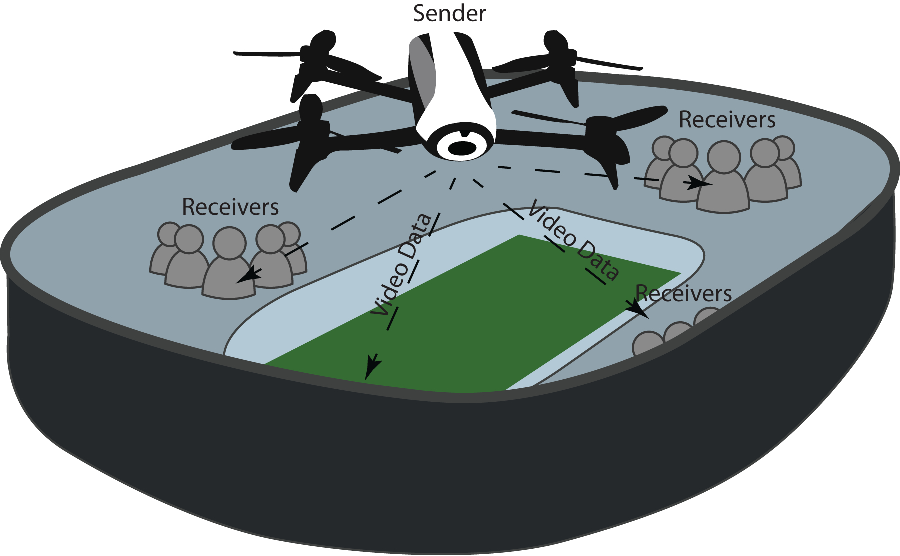
\includegraphics[width=\linewidth]{images/DroneIsolated.pdf}
  \caption{A drone multicasts a live video stream to spectators at a football stadium.}
  \label{fig:drone}
\end{figure}




%
%	One way to minimize the impact of packet erasures is to introduce an error control scheme that adapts based on the packet error rate (PER) \cite{rate_adapt_diff_rates}. Retransmission introduces some unwanted complexity and transmission overhead especially if packet erasures are uncorrelated. 
%	
%	
%	Prio art suggest erasure correction which is the ability to reobtain data after an erasure. Network Coding\cite{Ahlswede}, specifically Random Linear Network Coding (RLNC), shows great promise, and it has the capability to vary the resilience against erasures ad hoc \cite{nc_mult, HernándezMarcano2016}.
	%In wireless communication transmission errors are imminent and if the MAC layer detects an error the packet is erased. Since packets are not retransmitted in 802.11 multicast an error results in data loss at the receivers. There are two techniques for minimizing losses: error correction which is the ability to detect and correct an error within a packet and erasure correction which is the ability to reobtain data after a erasure.
	%since it not only possess error control properties but also allows for cooperative sharing and recovery of packets between the receiver.

	Transmission rate (TxR) adaptation schemes for multicast has been proposed in multiple papers \cite{SARM,rate_adapt_diff_rates,amuse}. Adaptation is desirable when the channel conditions change, e.g. when distance between the sender and receivers change. The authors of \cite{SARM} use signal to noise ratio to adapt the TxR, whereas \cite{rate_adapt_diff_rates} suggest a PER based adaptation. Adaptation of TxR and erasure code rely on feedback. In \cite{vid_rate,amuse} the authors provide solutions to gather feedback from multiple receivers. The authors of \cite{vid_rate} suggest collecting feedback from every receiver, while \cite{amuse} select a few receivers which send feedback periodically.

%	Feedback is required in order to adapt: RLNC, TxR and dealing with packet erasures. Implementing such a feature impose the following problem: how to get the feedback from multiple receivers and how to use it properly. In \cite{rate_adapt_diff_rates, amuse} the authors provide different solutions to the feedback problem. Since the feedback problem has several solutions, which does not affect the other reliability mechanisms, we assume the presence of a complete feedback system throughout the rest of this paper.
	Redundancy from the erasure code takes up usable resources from the TxR. Additionally, changing the TxR imposes limitations on how much video data can be serviced. This means that the video rate should be adjusted based on these limitations. Some applications require harder deadlines for video arrival and other applications require good video quality. Therefore, these requirements are additional parameters that should be considered when adjusting the video rate. 
	
% Our contribution
This paper examines reliable multicast for live video streaming from a drone. Inspired by \cite{vid_rate}, we form a policy that based on PER adapts transmission rate, erasure coding and video rate. We base our examination on the erasure coding random linear network coding (RLNC) \cite{randomnc} and the video encoding scheme H.264 \cite{H264}. In addition we account for video playback delay when considering two different playback methods, which to the best of our knowledge has not been considered in prior art. In particular, we customise the policies to work for drones by basing our investigation on channel throughput and video traces taken from a commercial drone, which has not been attempted previously. % The throughput examination assumes that every receiver's link to the drone is identical. 
%-----------
%	H.264 is a widely used video codec with hardware support and the ability to adjust the video bitrate \cite{H264}. We will base our analysis on this codec.
%
%	To sum up, the idea of a reliable multicast schemes is not a novel idea and there exists a plethora of research papers examining how the different features should be designed.
%	Based on the prior art the contribution of this paper is the following: We form a policy that describes how the TxR, RLNC, and video rate should be adjusted based on PER and the delay requirements of the application. The policy based on an experimental data trace collected with a consumer drone.
%------------

	The remainder of the paper is organized as follows. Section \ref{sec:methodmaterials} contains a description of the system and the scenario in which it operates. Section \ref{sec:impl} gives a brief presentation of implementation details on the three adaptable system components. Section \ref{sec:measure} describes the methods used for trace collection and system analysis. Section \ref{sec:results} contains the results of the measurements performed. Section \ref{sec:discussion} contains the resulting policy and the reasoning behind it. Section \ref{sec:conc} summarizes the policy, gives concluding remarks and future work.


	%A feedback system such as \cite{rate_adapt_diff_rates} propose that the transmitter multicasts probe packets at different rates and afterward request feedback from the individual users. However, such a system does not scale well due to the increase feedback communication overhead for each new receiver. To address the scalability problem a second paper\cite{amuse} propose an algorithm, Adaptive Multicast Service (AMuSe), which multiple receivers into smaller groups and assigning ``Feedback nodes'' which collects the feedback from other nodes in the same subgroup and delivers it to the service provider. This method lowers the actual feedback overhead to the transmitter and thereby improving the scalability.
